\chapter{Introduction}\label{ch:introduction}
One problem affecting 5\% of world population and approximately 15\% of adults aged 18 and over with and 
increasing rate with age which grows to almost 50\% for persons aged 75 and older is hearing loss.
This is quite an important impairment as it effects the quality of day to day life being harder for the 
individual to take part in social events and different daily activities. Besides the obvious problem of 
hearing loss is that about 16\% of adults aged between 20 and 69 years who could benefit from a hearing aid 
have never used one. This is partially because of the stigma that comes from using a hearing apparatus.
\cite{WHO}
 
 \begin{figure}[htp]
	\centering
	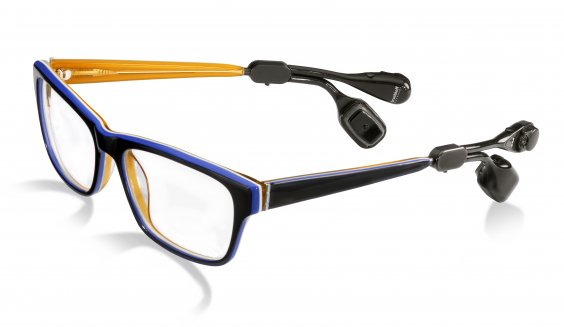
\includegraphics[width = 0.7\textwidth]{Illustrations/glasses_with_hearing_stuff.jpg}
	\caption{Bruckhoff Hearing Aid Glasses with Bone Conduction Technology}\cite{GLASSES}
	\label{fig:BoneConductionGlasses}
\end{figure}
 
By using a glasses frame with bone conduction technology this can be greatly improved, as glasses are more 
socially acceptable. Besides the social aspect, a glass frame can fit bigger batteries, more powerful 
electronics for digital filtering processing time and two microphones with which more complex filtering and 
speech recognition algorithms can be applied.

With all these being said, the project will involve two filtering methods using both microphones to achieve, 
theoretically, a better speech perception and understanding.

The first, involves using two microphones in order to record a two or 
more sound sources, from different angles.
With the sound samples recorded, the next step involves handling them 
in such a manner that allows to filter one source out, and keep the other.

Once one source has been filtered out, the next step is a neural network algorithm to filter the remaining 
noise from that direction and return a speech as clean and as clear as possible, in this way taking care of 
any noise that was happening in front or behind the person we want to hear more clearly.
\subsubsection{Reading Guide}
Chapter 2 deals with problem description and delimitation. 
Chapter 3 describes the set-up, components and methods used for recording samples.
Chapters 4 goes into detail about the signal processing techniques used during the project. Chapter 5 focuses on the separation of multiple sound sources.Chapter 6 describes the whole process and theory of creating the neural network used in the project. Chapter 7 and 
8 present a summary of the work done, suggest possible future uses of the research 
presented and draw a conclusion of the work carried out.